\documentclass[11pt,a4paper]{article}
\usepackage[T1]{fontenc}
\usepackage[utf8]{inputenc}
\usepackage{lmodern}
\usepackage[margin=2.5cm]{geometry}
\usepackage{amsmath,amssymb}
\usepackage{booktabs}
\usepackage{graphicx}
\usepackage[hidelinks]{hyperref}
\hypersetup{pdfauthor={Gianni Pilotti},pdftitle={Delta Hedging a Short Straddle and the VaR of the Hedged Book},pdfcreator={},pdfproducer={}}
\setlength{\parindent}{0pt}
\setlength{\parskip}{6pt}

\title{Delta Hedging a Short Straddle\\and the VaR of the Hedged Book}
\author{Gianni Pilotti}
\date{}

\begin{document}
\maketitle

\section{The Core Idea}
A delta-hedged option is not riskless. The hedge removes the first-order exposure to the underlying, and what is left is a bet on volatility: the seller collects implied variance through theta and pays realised variance through gamma. The repository tests this on SPY from 2011 to 2026, then asks a risk question: what is the one-day 99\% VaR of a book that has zero delta by construction?

\begin{itemize}
\item \textbf{Hedging:} a short at-the-money (ATM) straddle is opened every day, hedged daily at the close and held about 30 days.
\item \textbf{Surface:} historical option chains are not free, so the daily implied volatility surface is rebuilt from CBOE indices (VIX9D, VIX, VIX3M, SKEW, VVIX).
\item \textbf{VaR:} five methods are compared and backtested on the hedged book.
\end{itemize}

\section{Method}
\subsection{P\&L of a delta-hedged short option}
Each step, a delta-hedged short option earns
\[
d\Pi=-\tfrac12\,\Gamma S^2\left(\Big(\frac{dS}{S}\Big)^2-\sigma^2\,dt\right).
\]
The term $\sigma^2dt$ is the theta income. The squared return is the gamma cost. The trade makes money when realised variance is below implied variance. The code computes this sum along each path and compares it with the true hedged P\&L.

Two results are checked by Monte Carlo before using real data. The standard deviation of the hedging error with $N$ rebalances is, to leading order (Derman--Kamal),
\[
\mathrm{sd}\approx\sqrt{\frac{\pi}{4}}\;\mathcal{V}\,\frac{\sigma}{\sqrt N},
\]
where $\mathcal{V}$ is the vega of the option. With proportional costs, the repository also tests Leland's adjusted volatility.

\subsection{Volatility surface from CBOE indices}
The smile at maturity $T$ is
\[
\sigma(K,T)=\sigma_{atm}(T)\,\exp\!\left(\beta z+\tfrac12\gamma z^2\right),\qquad
z=3\tanh\!\left(\frac{\ln(K/F)}{3\,\sigma_{atm}\sqrt T}\right).
\]
\begin{itemize}
\item \textbf{Level:} $\sigma_{atm}(T)$ interpolates VIX9D, VIX and VIX3M (anchors at 9, 30 and 90 days) linearly in total variance $\sigma^2T$.
\item \textbf{Slope:} $\beta$ is solved so that the risk-neutral skewness of the log return equals $(100-\mathrm{SKEW})/10$. It is capped at the steepest slope that keeps the risk-neutral density non-negative.
\item \textbf{Curvature:} $\gamma=\mathrm{clip}(0.040\times\mathrm{VVIX}/0.86,\;0.01,\;0.09)$.
\item \textbf{Rescaling:} VIX is the fair strike of a 30-day variance swap, not the ATM volatility. The whole ATM level is multiplied by a factor $\lambda$ so that the smile's own variance swap, $\sqrt{\tfrac{2e^{rT}}{T}\int \mathrm{OTM}(K)/K^2\,dK}$, equals VIX.
\end{itemize}

\subsection{VaR of the hedged book}
The book is a short 30-day ATM straddle, hedged to zero delta and rebuilt every day. All methods use the same 500-day window of pairs (log return $x$, change in ATM vol $\Delta\sigma$), at $\alpha=99\%$. For each historical pair, with $\Delta S=S_0(e^{x}-1)$:

\begin{center}
\begin{tabular}{@{}lp{9.2cm}@{}}
\toprule
Method & Loss scenario \\
\midrule
Delta-normal & $z\,|\Delta_{book}|\,\mathrm{sd}(x)$, which is zero \\[2pt]
Delta-gamma-theta & $\tfrac12\Gamma\,\Delta S^2+\Theta\,\Delta t$ \\[2pt]
Delta-gamma-theta-vega & same, plus $\mathcal{V}\,\Delta\sigma$ \\[2pt]
Full revaluation, parallel shift & reprice the straddle at $(S_0+\Delta S,\ \sigma_{atm}+\Delta\sigma)$ at the old strike \\[2pt]
Full revaluation, smile & reprice at the old strike on the smile at the new spot, ATM level shifted by $\Delta\sigma$ \\
\bottomrule
\end{tabular}
\end{center}
The VaR is the empirical 1\% quantile of the loss scenarios, in \% of spot. The realised P\&L of the next day is the book repriced on the next day's smile. Two tests are used: Kupiec (exception count against 1\%) and Christoffersen (independence of exceptions). Both are compared with a $\chi^2_1$.

\section{Results}
\textbf{Simulation checks.} Hedging error with $\sigma=20\%$, a 30-day ATM call and 20,000 paths:

\begin{center}
\begin{tabular}{@{}rccc@{}}
\toprule
$N$ & Measured sd & Formula & Gap \\
\midrule
5 & 0.8363 & 0.9062 & $-7.7\%$ \\
21 & 0.4252 & 0.4422 & $-3.9\%$ \\
250 & 0.1266 & 0.1282 & $-1.2\%$ \\
\bottomrule
\end{tabular}
\end{center}
The formula is a leading-order result, so the gap shrinks as $N$ grows. A second test sells at 20\% while the path has 25\% volatility. Hedging at the realised volatility gives the same mean loss as hedging at the implied one ($-0.5719$ against $-0.5681$) with a much smaller standard deviation (0.1257 against 0.2709).

\textbf{SPY, 2011 to 2026.} One ATM straddle is sold every day and delta hedged at the close, with a half-spread of 0.5 vol point and 1 bp per stock trade:

\begin{center}
\begin{tabular}{@{}lc@{}}
\toprule
Metric & Value \\
\midrule
Trades (overlapping / non-overlapping) & 3,911 / 181 \\
Mean P\&L, in bp of strike & $-14$ \\
Win rate & 52.5\% \\
Same trades sold at the VIX level & $+67$ bp, win rate 80.8\% \\
Mean implied vs realised volatility & 14.7\% vs 14.7\% \\
$R^2$ of P\&L on the gamma-theta sum & 0.934 \\
$R^2$ of P\&L on implied minus realised vol & 0.597 \\
Worst trade & opened 9 Mar 2020, $-10.76\%$ \\
\bottomrule
\end{tabular}
\end{center}
The $+67$ bp comes from pricing the same trades at the VIX level, which sits above the ATM volatility when skew is negative, so it depends on the rescaling. At the rescaled ATM level the average trade loses 14 bp after costs. With 181 independent trades this is not distinguishable from zero. On two real SPX chains, the 30-day ATM volatility was 11.3\% (VIX 14.2\%) and 12.7\% (VIX 16.1\%). The rescaled surface gave 10.7\% and 12.1\%.

\begin{figure}[h]
\centering
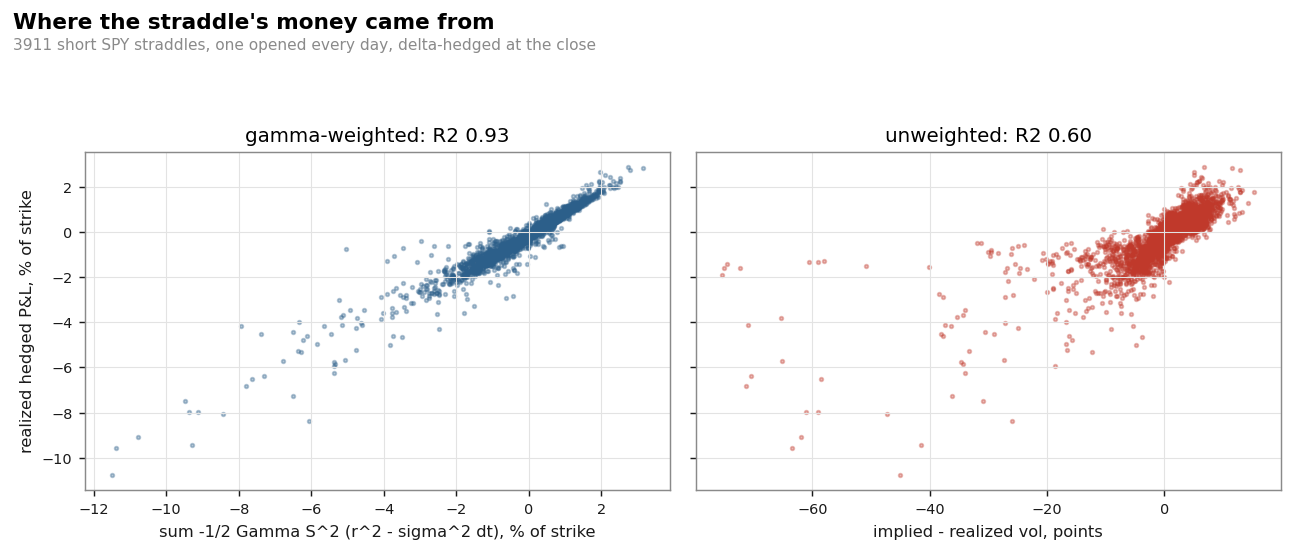
\includegraphics[width=0.86\textwidth]{../output/figures/hedge/spy_forecast.png}
\caption{Hedged P\&L of the 3,911 short straddles against the gamma-theta sum (left) and against implied minus realised volatility (right).}
\end{figure}

\textbf{VaR backtest.} 3,433 days from 2 January 2013 to 26 August 2026, 500-day window, 34.3 exceptions expected:

\begin{center}
\begin{tabular}{@{}lrrrr@{}}
\toprule
Method & Mean VaR (bp) & Exceptions & Rate (\%) & Kupiec $p$ \\
\midrule
Delta-normal & 0 & 1,495 & 43.55 & 0.000 \\
Delta-gamma-theta & 124 & 107 & 3.12 & 0.000 \\
Delta-gamma-theta-vega & 194 & 26 & 0.76 & 0.135 \\
Full revaluation, parallel & 178 & 29 & 0.84 & 0.348 \\
Full revaluation, smile & 158 & 39 & 1.14 & 0.433 \\
\bottomrule
\end{tabular}
\end{center}

\begin{itemize}
\item \textbf{Delta-normal:} the VaR is zero, so every losing day is an exception. It is a baseline only.
\item \textbf{Clustering:} the Christoffersen $p$-value is below 0.001 for all five methods.
\item \textbf{Ranking:} the order among the last three is not stable. Without the 17 days that touch a degenerate smile, only full revaluation on the smile passes Kupiec ($p=0.978$; the other two have $p=0.004$ and $0.025$). If the realised P\&L is repriced with a parallel vol shift, full revaluation on the smile fails (2.18\% exceptions).
\item \textbf{Worst days:} the largest realised losses (13.53\% on 24 March 2020) fall on days where the smile fit is degenerate, so they are model errors as much as market moves.
\end{itemize}

\section{Worked Example}
\textbf{One day of a hedged short straddle} (illustrative): $S=K=100$, $\sigma=20\%$, 30 days, $r=0$, one day $dt=1/365$. For the call, $\Gamma=0.06955$ and the straddle has $\Gamma=2\times0.06955=0.13910$.
\begin{align*}
\tfrac12\Gamma S^2 &= 0.5\times0.13910\times10{,}000=695.5,\\
\text{theta income} &= 695.5\times0.20^2/365=0.0762,\\
\text{move }+1\%:\quad & -695.5\times0.01^2+0.0762=-0.0696+0.0762=+0.0067,\\
\text{move }+2\%:\quad & -695.5\times0.02^2+0.0762=-0.2782+0.0762=-0.2020.
\end{align*}
The break-even daily move is $\sigma\sqrt{dt}=20\%/\sqrt{365}=1.05\%$.

\textbf{Derman--Kamal for the same option} with $N=21$: the call vega is $\mathcal{V}=11.43$, so $\mathrm{sd}=\sqrt{\pi/4}\times11.43\times0.20/\sqrt{21}=0.8862\times11.43\times0.20/4.583=0.442$ (0.4422 with unrounded inputs). This is the formula column above.

\textbf{Kupiec test} for full revaluation on the smile: $n=3433$, $x=39$, $p=0.01$, so 34.33 expected and $\hat p=1.136\%$.
\begin{align*}
\ln L_0&=3394\ln0.99+39\ln0.01=-213.7125,\\
\ln L_1&=3394\ln(1-\hat p)+39\ln\hat p=-213.4051,\\
LR&=-2\,(-213.7125+213.4051)=0.6147\;\Rightarrow\;p\text{-value}=0.433.
\end{align*}

\section{Limits}
\begin{itemize}
\item \textbf{Reconstructed smile:} only the ATM level and the index-implied smile are real data. On the checked chains, out-of-the-money puts come out up to 4 vol points too expensive and out-of-the-money calls up to 3 points too cheap.
\item \textbf{Skew constraint:} the SKEW target is matched exactly on 56\% of the 3,934 calibrated days. On the others the no-arbitrage bound binds.
\item \textbf{Circular backtest:} the realised P\&L is repriced on the same reconstructed surface that the full revaluation methods use, which favours them.
\item \textbf{SPY simplifications:} SPY is treated as European with no dividend yield, on unadjusted closes, so ex-dividend drops count as price moves.
\item \textbf{Window:} the 500-day window reacts slowly after a calm period. These are model outputs, not trading recommendations.
\end{itemize}

\end{document}
